
\documentclass[a4paper,11pt]{article}
\usepackage[a4paper, margin=8em]{geometry}

% usa i pacchetti per la scrittura in italiano
\usepackage[french,italian]{babel}
\usepackage[T1]{fontenc}
\usepackage[utf8]{inputenc}
\frenchspacing 

% usa i pacchetti per la formattazione matematica
\usepackage{amsmath, amssymb, amsthm, amsfonts}

% usa altri pacchetti
\usepackage{gensymb}
\usepackage{hyperref}
\usepackage{standalone}

% imposta il titolo
\title{Appunti Fondamenti di Automatica}
\author{Luca Seggiani}
\date{2025}

% disegni
\usepackage{pgfplots}
\pgfplotsset{width=10cm,compat=1.9}

% imposta lo stile
% usa helvetica
\usepackage[scaled]{helvet}
% usa palatino
\usepackage{palatino}
% usa un font monospazio guardabile
\usepackage{lmodern}

% tikz in sans
\tikzset{every picture/.style={/utils/exec={\sffamily}}}

\renewcommand{\rmdefault}{ppl}
\renewcommand{\sfdefault}{phv}
\renewcommand{\ttdefault}{lmtt}

% circuiti
\usepackage{circuitikz}
\usetikzlibrary{babel}

% disponi il titolo
\makeatletter
\renewcommand{\maketitle} {
	\begin{center} 
		\begin{minipage}[t]{.8\textwidth}
			\textsf{\huge\bfseries \@title} 
		\end{minipage}%
		\begin{minipage}[t]{.2\textwidth}
			\raggedleft \vspace{-1.65em}
			\textsf{\small \@author} \vfill
			\textsf{\small \@date}
		\end{minipage}
		\par
	\end{center}

	\thispagestyle{empty}
	\pagestyle{fancy}
}
\makeatother

% disponi teoremi
\usepackage{tcolorbox}
\newtcolorbox[auto counter, number within=section]{theorem}[2][]{%
	colback=blue!10, 
	colframe=blue!40!black, 
	sharp corners=northwest,
	fonttitle=\sffamily\bfseries, 
	title=Teorema~\thetcbcounter: #2, 
	#1
}

% disponi definizioni
\newtcolorbox[auto counter, number within=section]{definition}[2][]{%
	colback=red!10,
	colframe=red!40!black,
	sharp corners=northwest,
	fonttitle=\sffamily\bfseries,
	title=Definizione~\thetcbcounter: #2,
	#1
}

% disponi problemi
\newtcolorbox[auto counter, number within=section]{problem}[2][]{%
	colback=green!10,
	colframe=green!40!black,
	sharp corners=northwest,
	fonttitle=\sffamily\bfseries,
	title=Problema~\thetcbcounter: #2,
	#1
}

% disponi codice
\usepackage{listings}
\usepackage[table]{xcolor}

\lstdefinestyle{codestyle}{
	backgroundcolor=\color{black!5}, 
	commentstyle=\color{codegreen},
	keywordstyle=\bfseries\color{magenta},
	numberstyle=\sffamily\tiny\color{black!60},
	stringstyle=\color{green!50!black},
	basicstyle=\ttfamily\footnotesize,
	breakatwhitespace=false,         
	breaklines=true,                 
	captionpos=b,                    
	keepspaces=true,                 
	numbers=left,                    
	numbersep=5pt,                  
	showspaces=false,                
	showstringspaces=false,
	showtabs=false,                  
	tabsize=2
}

\lstdefinestyle{shellstyle}{
	backgroundcolor=\color{black!5}, 
	basicstyle=\ttfamily\footnotesize\color{black}, 
	commentstyle=\color{black}, 
	keywordstyle=\color{black},
	numberstyle=\color{black!5},
	stringstyle=\color{black}, 
	showspaces=false,
	showstringspaces=false, 
	showtabs=false, 
	tabsize=2, 
	numbers=none, 
	breaklines=true
}

\lstdefinelanguage{javascript}{
	keywords={typeof, new, true, false, catch, function, return, null, catch, switch, var, if, in, while, do, else, case, break},
	keywordstyle=\color{blue}\bfseries,
	ndkeywords={class, export, boolean, throw, implements, import, this},
	ndkeywordstyle=\color{darkgray}\bfseries,
	identifierstyle=\color{black},
	sensitive=false,
	comment=[l]{//},
	morecomment=[s]{/*}{*/},
	commentstyle=\color{purple}\ttfamily,
	stringstyle=\color{red}\ttfamily,
	morestring=[b]',
	morestring=[b]"
}

% disponi sezioni
\usepackage{titlesec}

\titleformat{\section}
{\sffamily\Large\bfseries} 
{\thesection}{1em}{} 
\titleformat{\subsection}
{\sffamily\large\bfseries}   
{\thesubsection}{1em}{} 
\titleformat{\subsubsection}
{\sffamily\normalsize\bfseries} 
{\thesubsubsection}{1em}{}

% disponi alberi
\usepackage{forest}

\forestset{
	rectstyle/.style={
		for tree={rectangle,draw,font=\large\sffamily}
	},
	roundstyle/.style={
		for tree={circle,draw,font=\large}
	}
}

% disponi algoritmi
\usepackage{algorithm}
\usepackage{algorithmic}
\makeatletter
\renewcommand{\ALG@name}{Algoritmo}
\makeatother

% disponi numeri di pagina
\usepackage{fancyhdr}
\fancyhf{} 
\fancyfoot[L]{\sffamily{\thepage}}

\makeatletter
\fancyhead[L]{\raisebox{1ex}[0pt][0pt]{\sffamily{\@title \ \@date}}} 
\fancyhead[R]{\raisebox{1ex}[0pt][0pt]{\sffamily{\@author}}}
\makeatother

\begin{document}

% sezione (data)
\section{Lezione del 30-04-25}

% stili pagina
\thispagestyle{empty}
\pagestyle{fancy}

% testo
\subsection{Criterio di Nyquist}
Il criterio di Nyquist è un metodo per studiare nel piano complesso l'effetto della reazione negativa sui poli del sistema in catena chiusa con controllore a partire dalla conoscenza della funzione di trasferimento in catena aperta.

Vediamo quindi la struttura della catena chiusa nel dettaglio.
Diciamo che il sistema è definito dalla funzione di trasferimento $G(s)$, che è controllato dal controllore $C(s)$ e si trova in un ciclo di retroazione del tipo che abbiamo già visto:
\begin{center}
	\begin{tikzpicture}
		\draw (1,0) rectangle (3, 1);
		\node at (2, 0.5) {$G(s)$};

		\draw (-3,0) rectangle (-1, 1);
		\node at (-2, 0.5) {$C(s)$};

		\draw[-stealth] (-7, 0.5) -> (-5.1, 0.5);
		\draw[-stealth] (-5, 0.5) -> (-3, 0.5);
		\draw[-stealth] (-1, 0.5) -> (1, 0.5);
		\draw[-stealth] (3, 0.5) -> (7, 0.5);

		\draw (5, 0.5) -> (5, -1);
		\draw (5, -1) -> (-5, -1);
		\draw[-stealth] (-5, -1) -> (-5, 0.5);

		\draw[fill=white] (-5, 0.5) circle (0.1);

		\node at (-6, 0.75) {$w$};
		\node at (6, 0.75) {$y$};

		\node at (-4.75, 0.75) {$+$};
		\node at (-4.75, 0.25) {$-$};

		\node at (0, 0.75) {$u$};
		\node at (-3.8, 0.75) {$e$};
	\end{tikzpicture}
\end{center}

Da cui si calcola la risposta complessiva $G_{cc}(s)$, prendendo il sistema:
\[
	\begin{cases}
		G_{cc}(s) = \frac{y}{w} \\ 
		y = u \cdot G(s) = e \cdot C(s) G(s) \\ 
		e = w - y
	\end{cases}
\]
e risolvendo come:
$$
y = (w - y) C(s) G(s) \, \Rightarrow \, y = \frac{w \cdot C(s) G(s)}{1 + C(s)G(s)} \, \Rightarrow \, G_{cc}(s) = \frac{C(s) G(s)}{1 + C(s)G(s)}
$$
che è la classica funzione di trasferimento a ciclo chiuso a cui siamo abituati.
Per ora assumeremo che il controllore $C(s)$ sarà proporzionale, cioè rappresentato da una costante $K_C$, per cui:
$$
G_{cc}(s) = \frac{K_C \cdot G(s)}{1 + K_C \cdot G(s)} = \frac{\hat{G}(s)}{1 + \hat{G}(s)}
$$
chiamando $\hat{G}(s) = C(s) G(s) = K_C \cdot G(s)$.

La stabilità del sistema in ciclo chiuso $G_{cc}(s)$ sarà quindi data dalle radici dell'equazione caratteristica:
$$
1 + \hat{G}(s) = 0
$$
cioè dai poli in ciclo chiuso.

A questo punto esplicitiamo il polinomio caratteristico, nota la forma generica di $G(s)$:
$$
G(s) = K_G \frac{ \prod_{i=1}^m (s - z_i) }{ \prod_{i=1}^n (s - p_i) }
$$
come:
$$
1 + \hat{G}(s) = 1 + K \frac{ \prod_{i = 1}^m (s - z_i) }{ \prod_{i = 1}^n (s - p_i) } = \frac{ K \prod_{i = 1}^m (s - z_i) + \prod_{i = 1}^n (s - p_i) }{ \prod_{i = 1}^n }
$$
con $K = K_C K_G$.
Ci accorgiamo quindi di 3 cose:
\begin{itemize}
	\item Ci interessa la risposta armonica, quindi potremo porre $s = j\omega$;
	\item Il denominatore sarà la somma di due polinomi $p_1$ e $p_2$, di grado rispettivamente $m$ e $n$.
		Faremo l'assunto $m \leq n$ (che è comunque condizione di stabilità), per cui avremo che il denominatore sarà rappresentato complessivamente da un singolo polinomio di grado $n$:
		$$
		\prod_{i = 1}^n (s - r_i)
		$$
		le cui radici $r_i$ sono esattamente i poli in ciclo chiuso;
	\item I polinomi che avremo a numeratore e denominatore saranno entrambi \textit{monici}.
\end{itemize}
Da questo potremo riscrivere come:
$$
1 + \hat{G}(s) = \alpha \frac{\prod_{i = 1}^n (j \omega - r_i)}{\prod_{i = 1}^n (j \omega - p_i)}
$$
dove $\alpha$ è una costante di proporzionalità.
Per calcolarla ci accorgiamo che dalla terza osservazione:
$$
\lim_{\omega \rightarrow \infty} \frac{\prod_{i = 1}^n (j \omega - r_i)}{\prod_{i = 1}^n (j \omega - p_i)} = 1
$$
per cui basterà far combaciare il limite ad infinito:
$$
\lim_{\omega \rightarrow \infty} 1 + \hat{G}(j \omega) = 1 + K \frac{ \prod_{i = 1}^m (j \omega - z_i) }{ \prod_{i = 1}^n (j \omega - p_i) } =
\begin{cases}
	1 \quad m < n \\ 
	1 + K \quad m = n
\end{cases}
$$
per cui:
\[
	\alpha = 1 + \hat{G}(\infty) =			
	\begin{cases}
		1, \quad m < n \\
		1 + K, \quad m = n
	\end{cases}
\]

Vorremo allora imporre le seguenti condizioni di stabilità riguardo ai poli in ciclo chiuso:
\begin{enumerate}
	\item Nessuna radice deve andare nel semipiano $\mathrm{Re}(r_i) > 0$ al variare del guadagno $K_C$;
	\item $\hat{G}(j \omega) \neq -1$.
\end{enumerate}

L'idea sarà di trovare il modo di affermare se tali condizioni sono soddisfatte per il ciclo chiuso guardando alla catena aperta, sfruttando il fatto che fra il polinomio caratteristico $1 + \hat{G}(s)$ (che ci dà i poli in catena chiusa) e la funzione di trasferimento in catena aperta $\hat{G}(s)$ esiste una relazione:
$$
1 + \hat{G}(s) \sim \hat{G}(s)
$$
cioè tracciare il diagramma di Nyquist del polinomio caratteristico equivale a traslare il diagramma di Nyquist della funzione di trasferimento in catena aperta verso destra di $1$.

In questo abbiamo due metodi, che si basano entrambi sull'osservare alcune proprietà fondamentali del diagramma di Nyquist:
\begin{enumerate}
	\item 
		Nota la loro forma, potremmo ricavare una condizione sugli angoli che i punti di $1 + \hat{G}(j\omega)$ spazzano con poli e zeri passando per $j\omega$, con $\omega$ che parte da $-\infty$ e arriva a $+\infty$:
		\begin{center}
			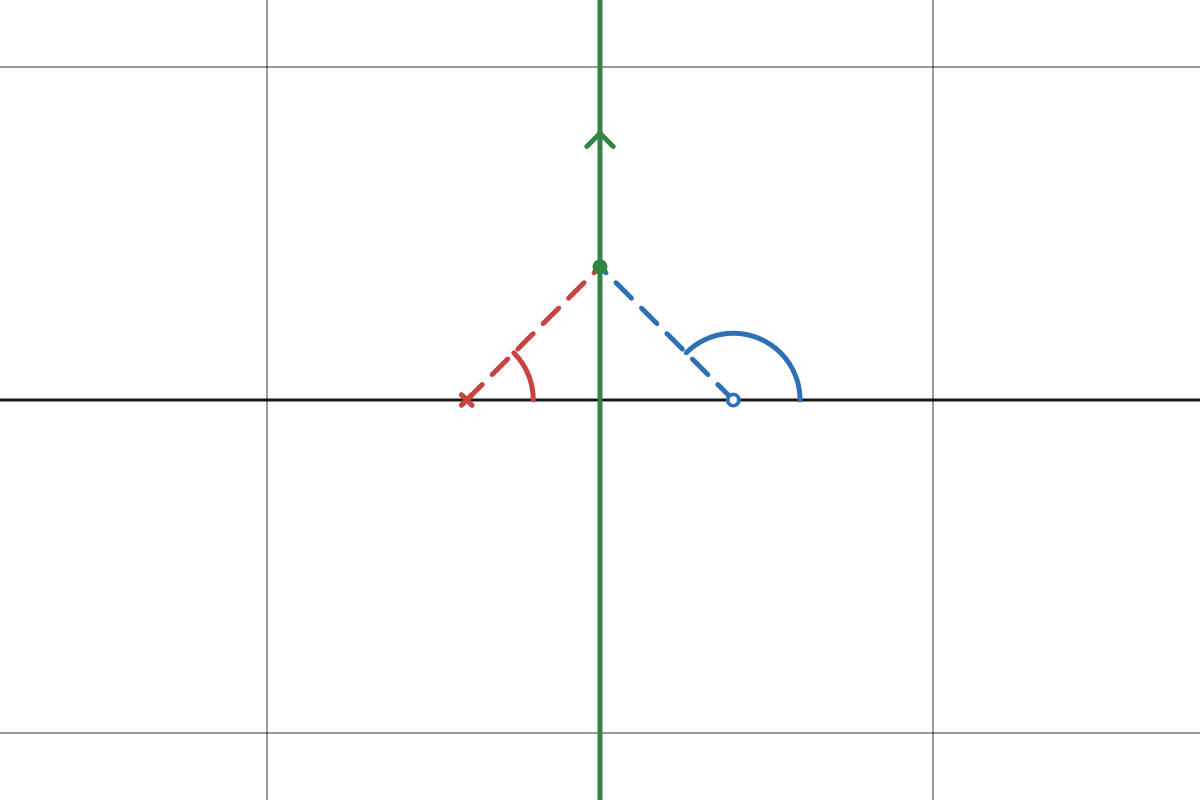
\includegraphics[scale=0.28]{../figures/nyq_crit_m1.png}
		\end{center}
		Questi saranno le fasi dei cosiddetti punti del \textit{diagramma di Nyquist completo}, cioè che prevede $\omega \in (-\infty, +\infty)$ e non solo $\omega \in [0, +\infty]$.
	
		\noindent
		
		\begin{minipage}{\textwidth}

		Notiamo che, per i poli sull'asse complesso, questi si evitano passando alla loro \textit{destra}:
		\begin{center}
			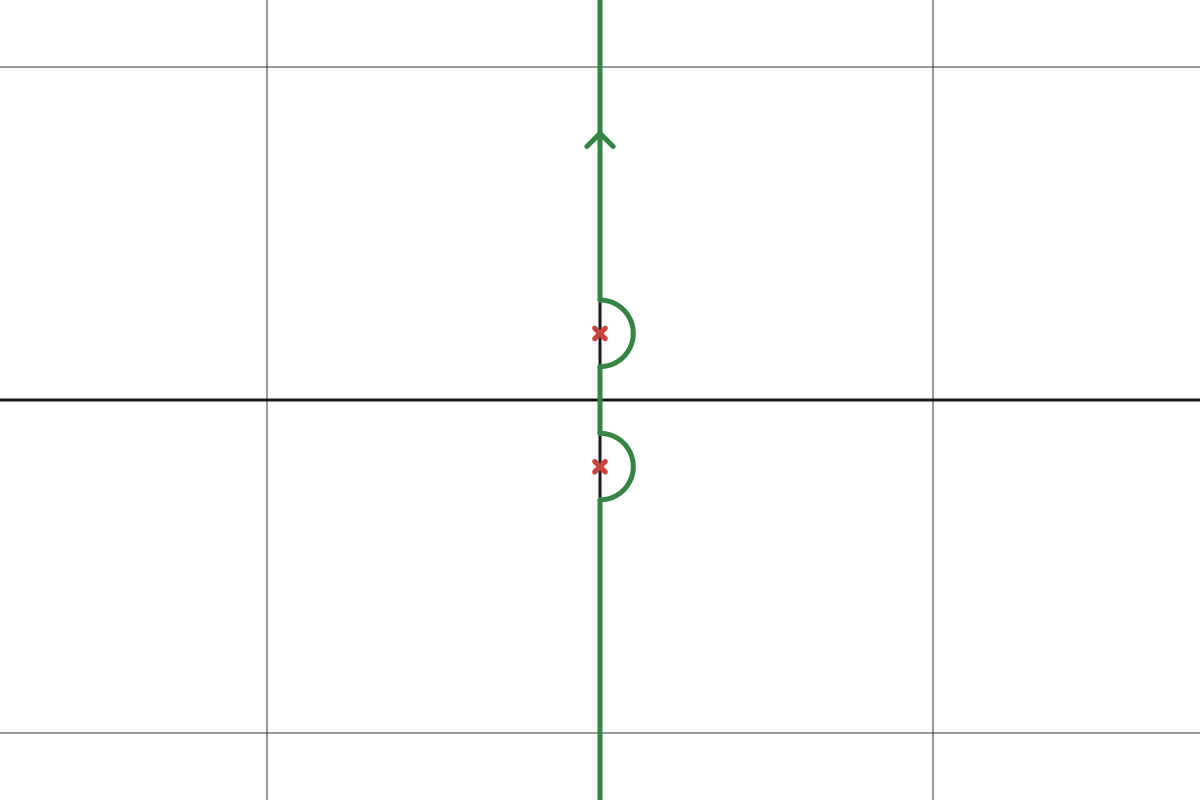
\includegraphics[scale=0.28]{../figures/nyq_crit_ip.png}
		\end{center}

		\end{minipage}

		A questo punto potremo affermare che:
		\begin{itemize}
			\item Riguardo ai poli si ha:
				\begin{itemize}
					\item I poli a parte reale negativa portano a variazione di fase $-\pi$;
					\item I poli a parte reale nulla portano a variazione di fase $-\pi$;
					\item I poli a parte reale positiva portano a variazione di fase $+\pi$.
				\end{itemize}
			\item Riguardo agli zeri si ha:
				\begin{itemize}
					\item Gli zeri a parte reale negativa portano a variazione di fase $+\pi$;
					\item Gli zeri a parte reale positiva portano a variazione di fase $-\pi$.
				\end{itemize}
		\end{itemize}

		Questo viene direttamente dal tracciamento degli angoli dei poli e degli zeri in catena chiusa con i punti sull'asse immaginario positivo:

		Chiaramente l'unico punto esente da questa condizione è quello $\hat{G}(j \omega) = -1$, in quanto in tal caso diventa impossibile definire il vettore fra i poli in catena chiusa e il punto sull'asse immaginario.
		Abbiamo però che questo è il punto che annulla il denominatore della catena chiusa $G_{cc}(s)$, e quindi lo escludiamo a prescindere.

		Definiamo quindi, riguardo all'espressione del polinomio caratteristico appena trovata:
		$$
		1 + \hat{G}(s) = \alpha \frac{ \prod_{i = 1}^n (j \omega - r_i) }{ \prod_{i = 1}(j \omega - p_i) }
		$$
		i valori:
		\begin{itemize}
			\item $R^{(+)} =$ numero di radici a parte reale positiva;
			\item $R^{(-)} =$ numero di radici a parte reale negativa;
			\item $P^{(+)} =$ numero di poli a parte reale positiva;
			\item $P^{(-)} =$ numero di poli a parte reale negativa;
			\item $P^{(0)} =$ numero di poli sull'asse immaginario.
		\end{itemize}
		Varranno le identità:
		\[
			\begin{cases}
				R^{(+)} + R^{(-)} = m \\
				P^{(+)} + P^{(-)} + P^{(0)} = n
			\end{cases}
		\]
		e la variazione totale di fase sarà:
		$$
		\angle 1 + \hat{G}(j \omega) = R^{(+)} \cdot - \pi + R^{(-)} \cdot \pi + P^{(+)} \cdot \pi + P^{(-)} \cdot - \pi + P^{(0)} \cdot - \pi
		$$
		da cui:
		$$
		\angle 1 + \hat{G}(j \omega) = \pi \left( -R^{(+)} + R^{(-)} + P^{(+)} - P^{(-)} - P^{(0)} \right) 
		= \pi \left( n - 2 R^{(+)} - n + 2 \cdot P^{(+)} \right)
		$$
		cioè la variazione di fase non dipende dall'ordine $n$ del sistema, ma solo da dove si trovano i poli e le radici a parte reale positiva, e in particolare vale:
		$$
		\angle 1 + \hat{G}(j \omega) = 2 \pi \left( P^{(+)} - R^{(+)} \right)
		$$
		A questo punto basterà imporre la condizione di stabilità $R^{(+)} = 0$ (ricordiamo che gli zeri/radici del polinomio caratterstico equivalgono ai poli del sistema in ciclo chiuso), per cui:
		$$
		N_{ao} = P^+
		$$
		dove $N_{ao}$ è il numero di giri in senso antiorario attorno al punto critico, che per $1 + \hat{G}(j\omega)$ era l'origine e per il comune diagramma di Nyquist della catena aperta sarà $-1$ (o $-\frac{1}{K}$ se la catena aperta è $K \cdot G(j\omega)$).

	\item 
		Altrimenti basterà considerare il cosiddetto \textbf{percorso di Nyquist}, cioè quel percorso che parte da $0$, arriva a $+\infty$ e si ricongiunge \textit{all'infinto}, sul lato destro del piano complesso, a $-\infty$ per tornare a 0:
		\begin{center}
			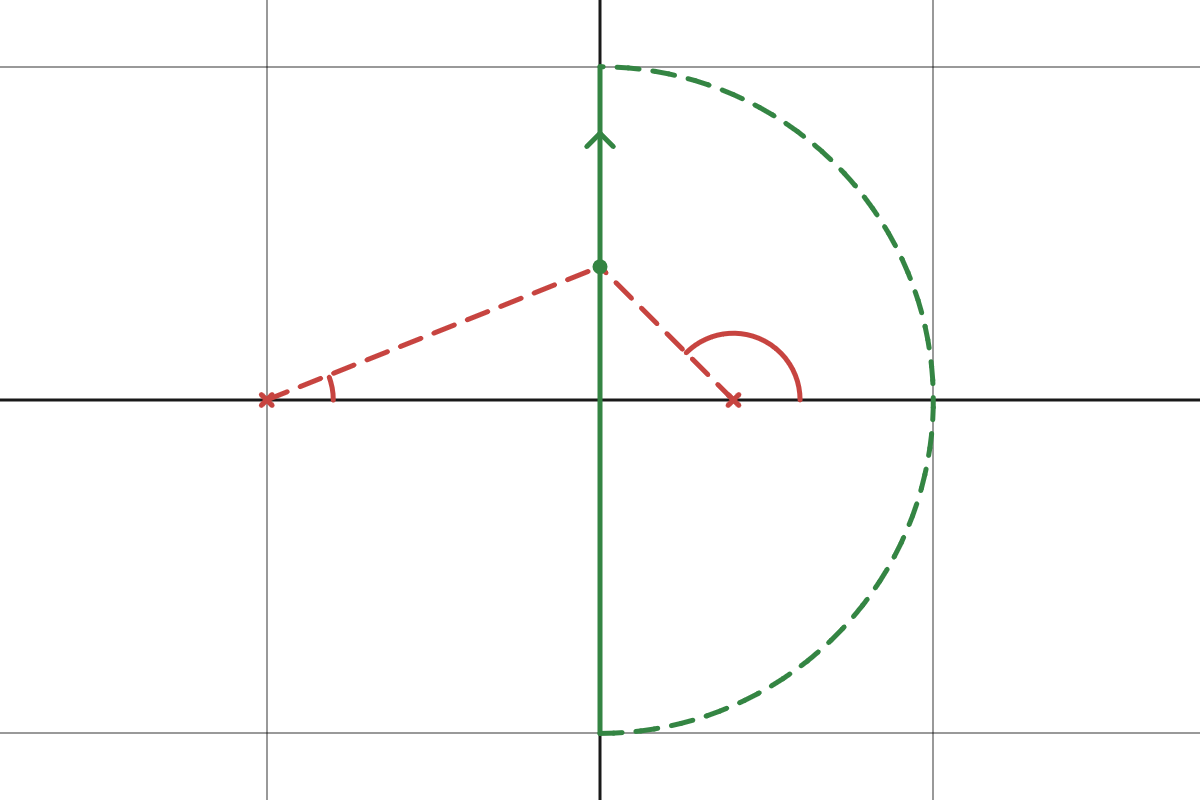
\includegraphics[scale=0.28]{../figures/nyq_crit_m2.png}
		\end{center}
		Come per il percorso considerato prima, si passa a \textit{destra} dei poli sull'asse complesso.

		In questo caso sarà immediato verificare che i soli poli o zeri che contribuiscono alla fase per un giro completo sono quelli interni a tale percorso, e per la precisione:
		\begin{itemize}
			\item I poli a parte reale positiva portano a variazione di fase $+2\pi$;
			\item Gli zeri a parte reale positiva portano a variazione di fase $-2\pi$;
			\item Tutti gli altri punti portano a variazione di fase $0$.
		\end{itemize}

		Da questo si avrà quindi la formula complessiva:
		$$
		\angle 1 + \hat{G}(j\omega) = 2\pi \left( P^{(+)} - R^{(+)} \right)
		$$
		con:
		\begin{itemize}
			\item $R^{(+)} = $ numero di radici a parte reale positiva;
			\item $P^{(+)} = $ numero di poli a parte reale positiva.
		\end{itemize}
		che è la stessa relazione di prima, per cui si ottiene lo stesso risultato.
\end{enumerate}

\end{document}
